\chapter{Hardware}

Con el ánimo de tener una plataforma real sobre la que probar el rendimiento de los algoritmos de control diseñados, se ha diseñado y construido un cuadrirrotor \textit{ad hoc} para este propósito. Un cuadricóptero convencional cuenta con: un chasis o cuadro que lo sustenta, cuatro motores y la electrónica necesaria para controlarlos, una controladora de vuelo que lo comanda y baterías que le proporcionan energía.

\begin{figure}[htb!]
	\centering
	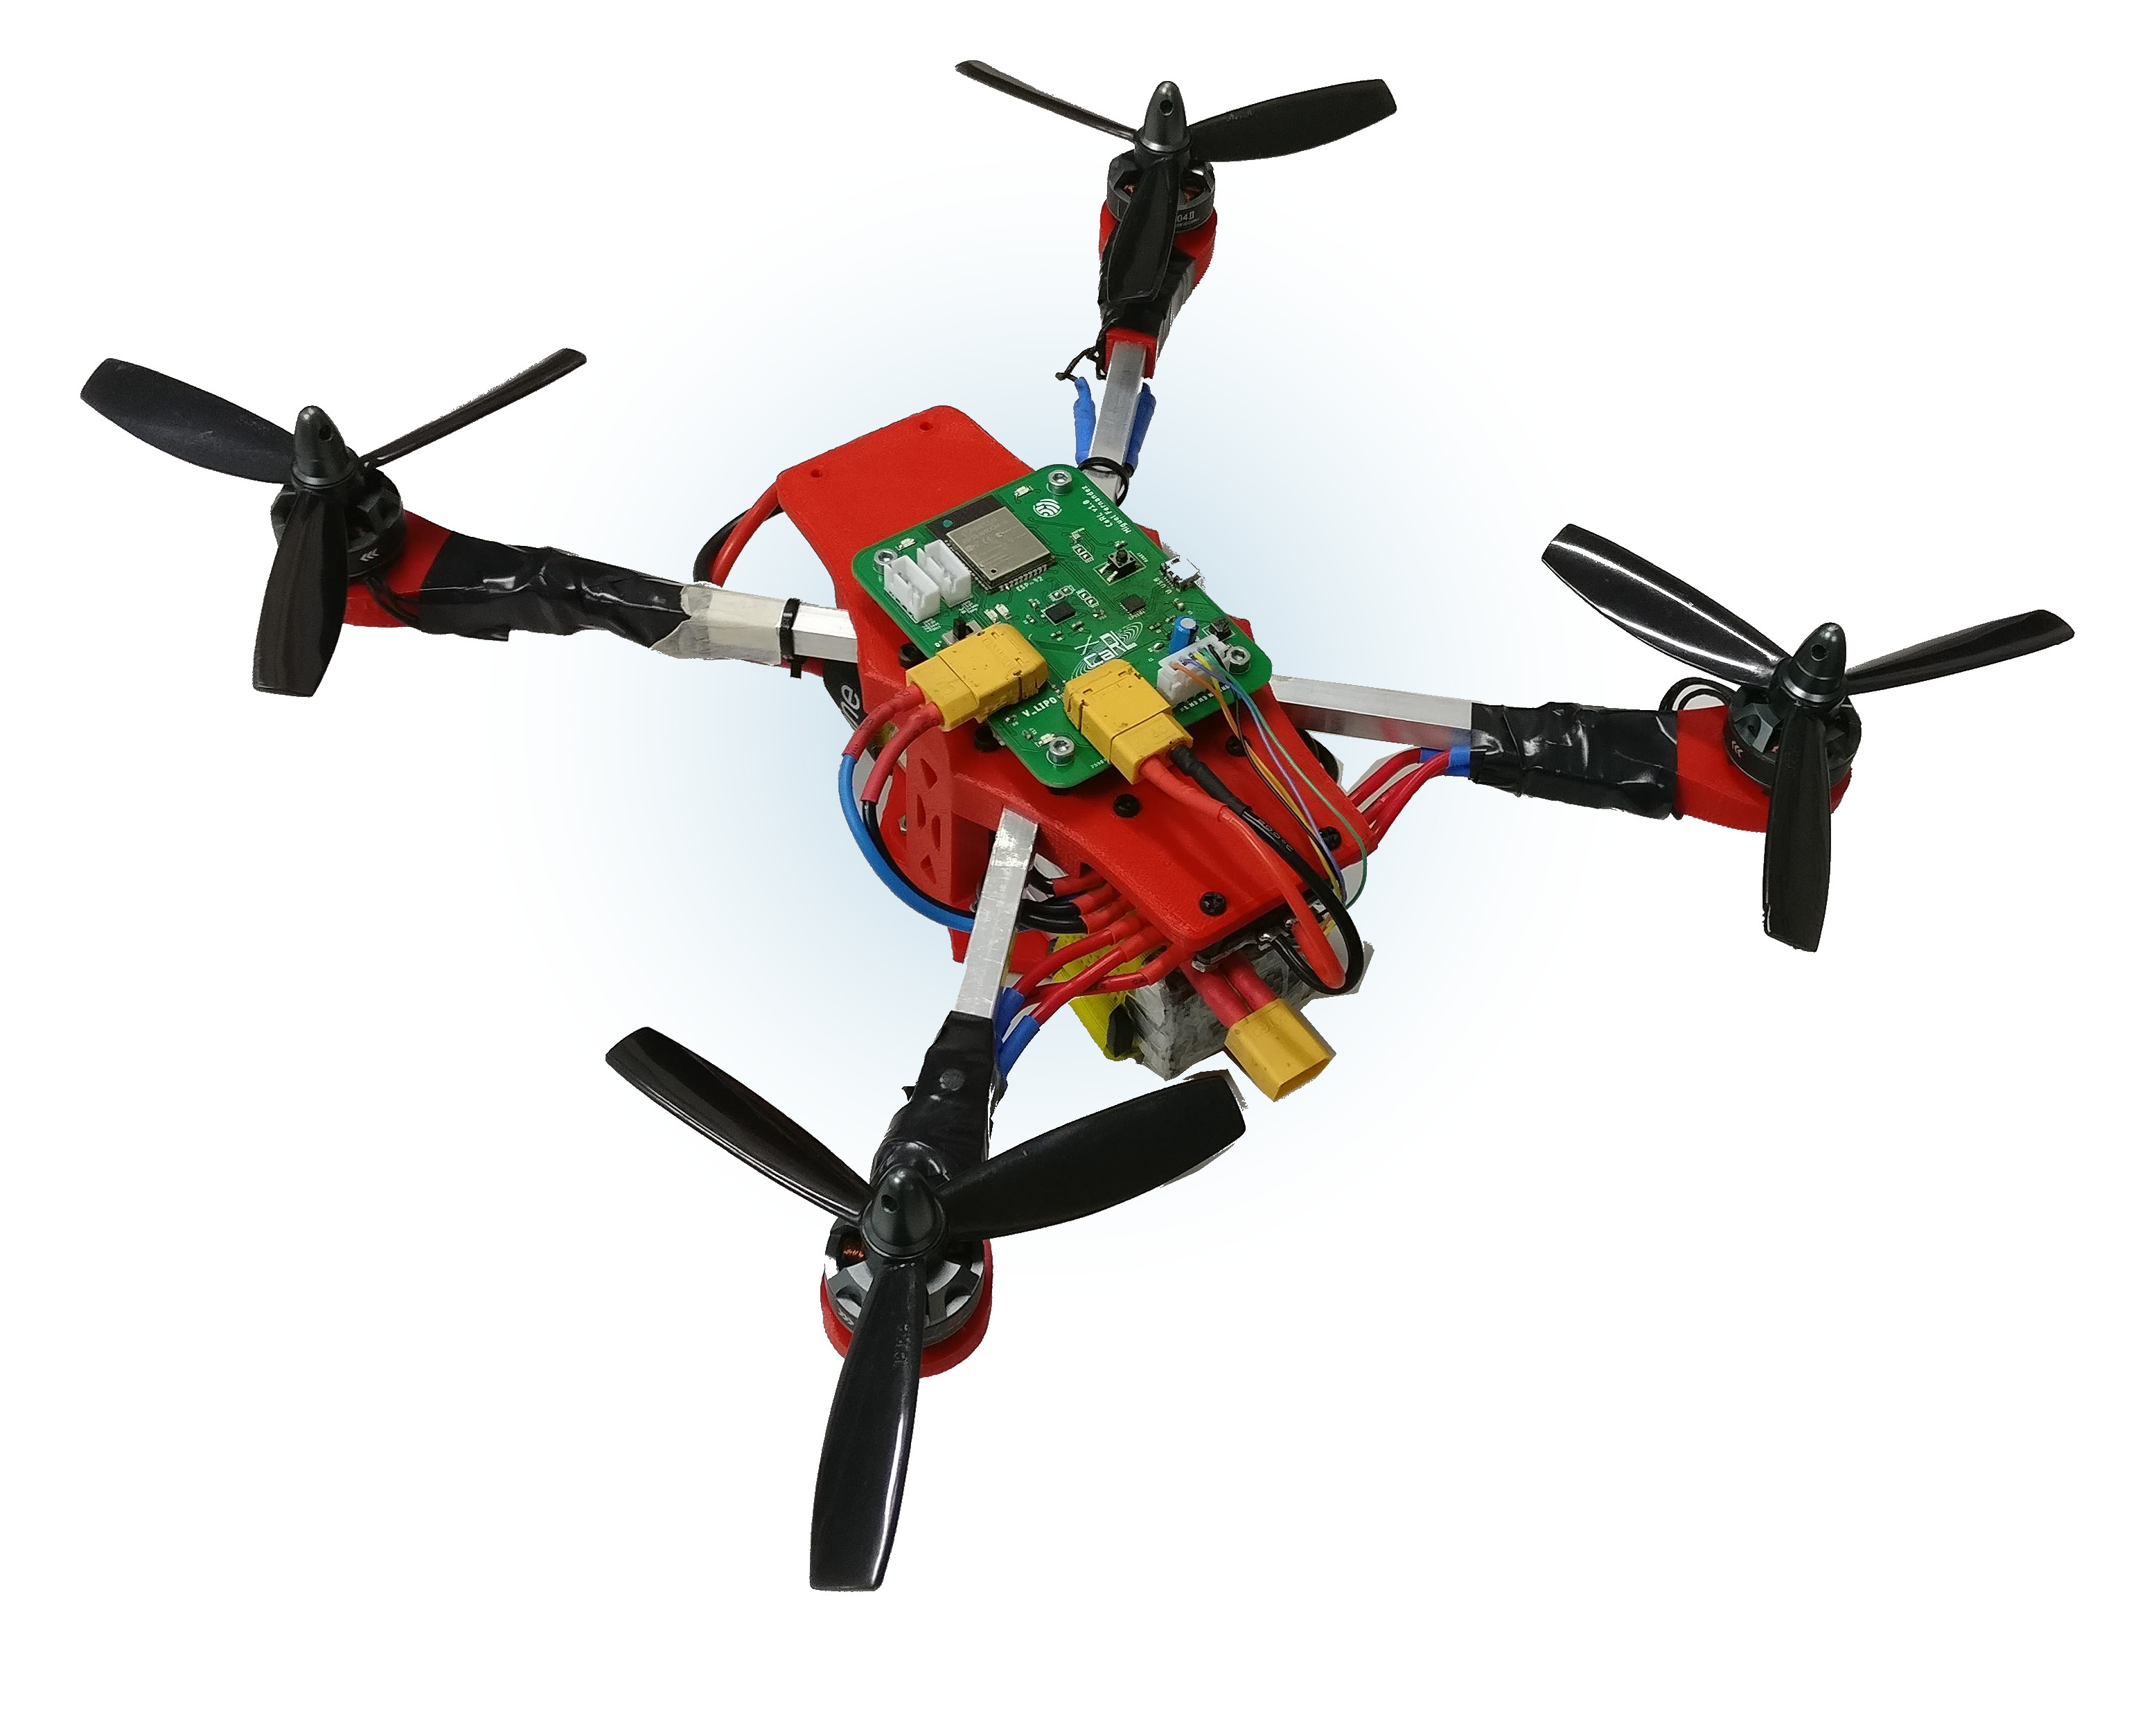
\includegraphics[width=0.95\textwidth]{hardware/droneImg}
	\caption{Cuadricóptero diseñado con el autopiloto incoporado. }
	\label{hardware:droneImg}
\end{figure}

\begin{figure}[htb!]
	\centering
	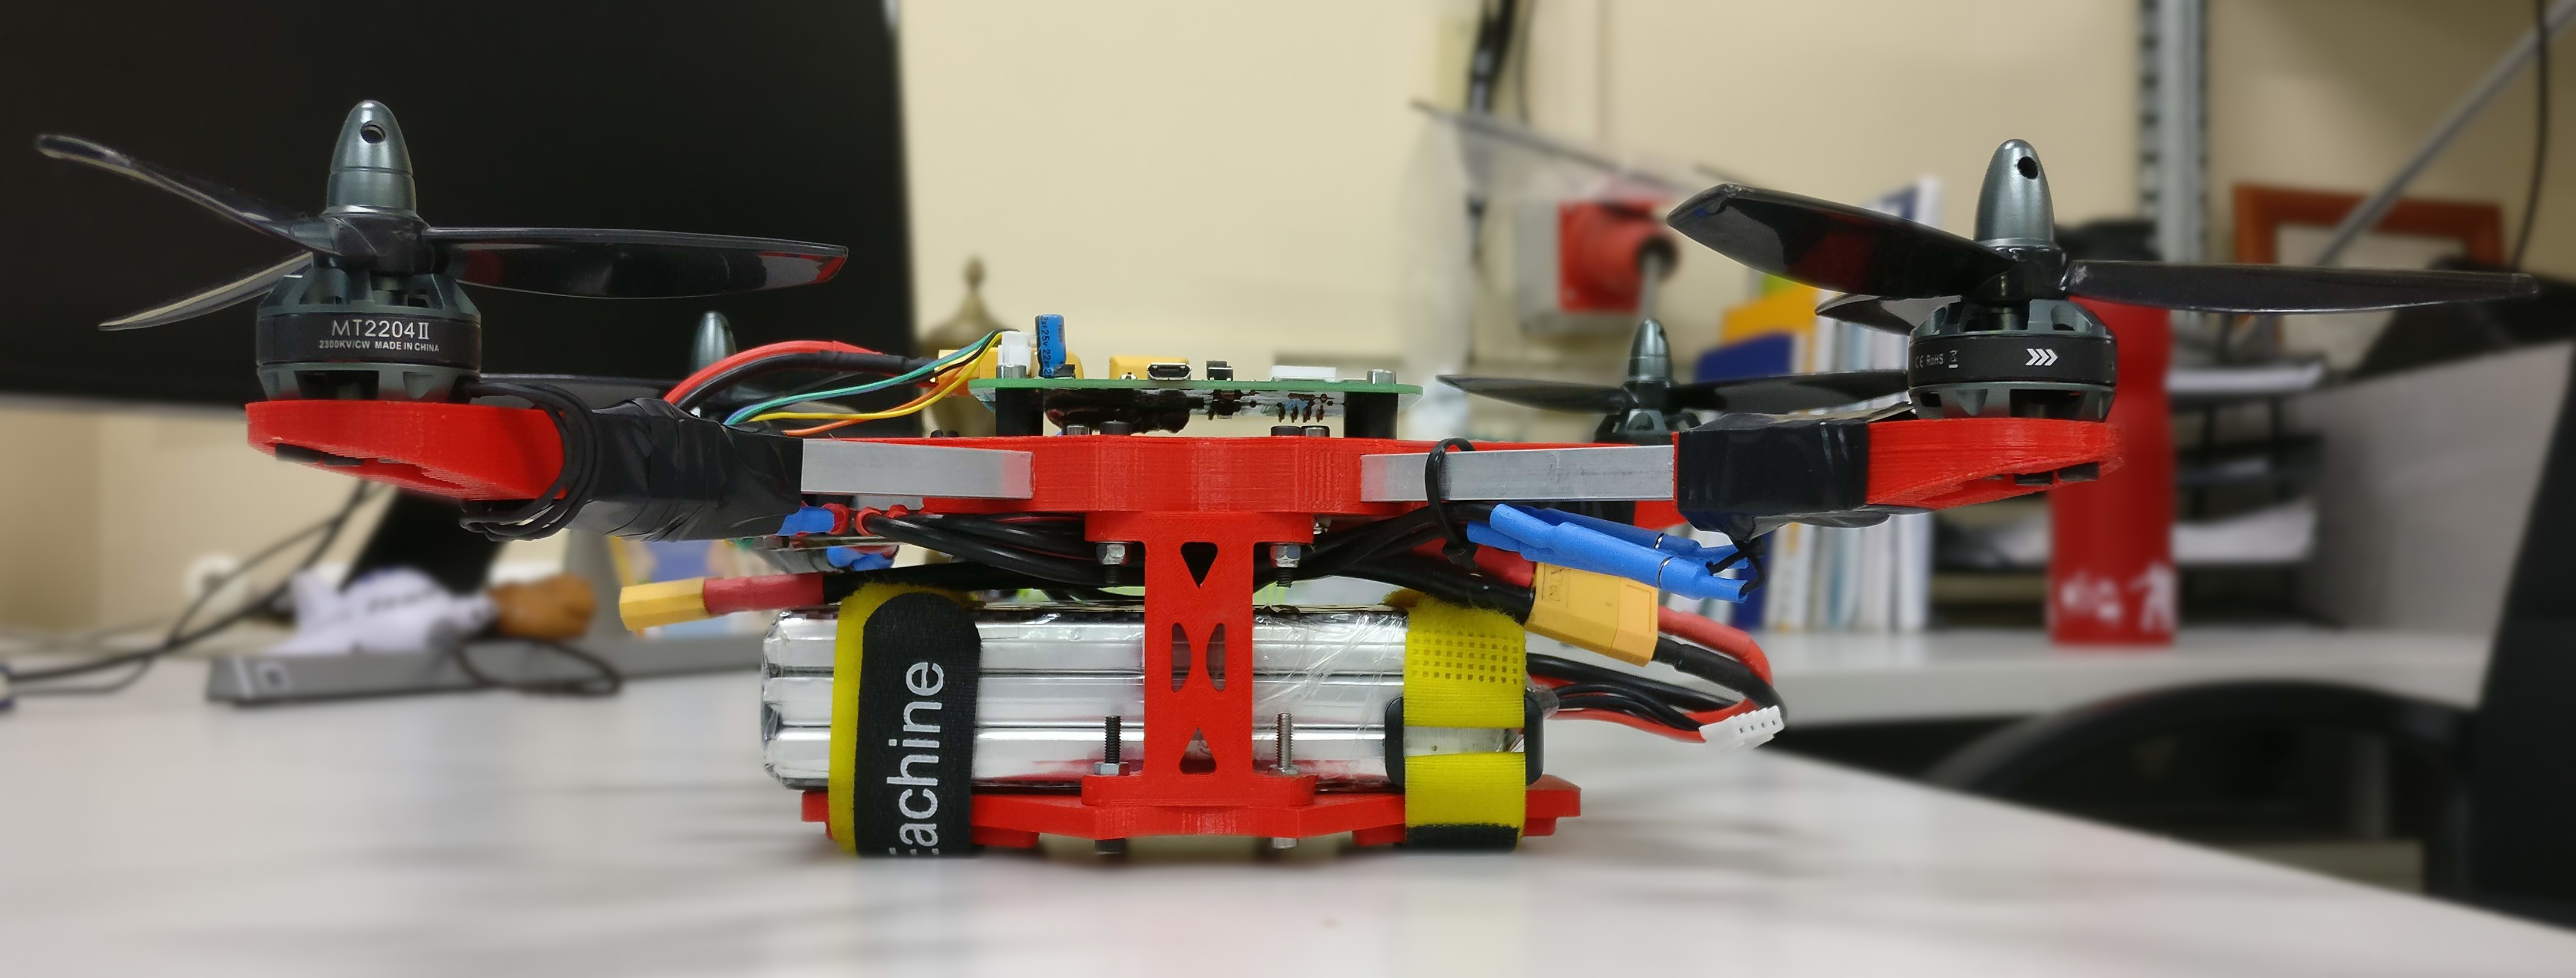
\includegraphics[width=0.95\textwidth]{hardware/Drones_side}
	\caption{Cuadricóptero diseñado con el autopiloto incoporado.}
	\label{hardware:droneImg}
\end{figure}


A continuación se detallará como son las distintas partes físicas del dron que se ha fabricado.



\section{Cuadro}
El \textit{frame} está compuesto por perfiles de aluminio y piezas de PLA fabricadas mediante impresión 3D de diseño propio. La estructura básica está formada por 5 conjuntos de piezas distintos:
\begin{itemize}
	\item[$\bullet$] \textbf{Portamotores}: son las piezas donde se alojan los motores. Para conseguir una buena fijacion los motores se atornillan a los portamotores empleando 4 tornillos dispuestos seǵun los vértices de un rombo.
	
	\begin{figure}[htb!]
		\centering
		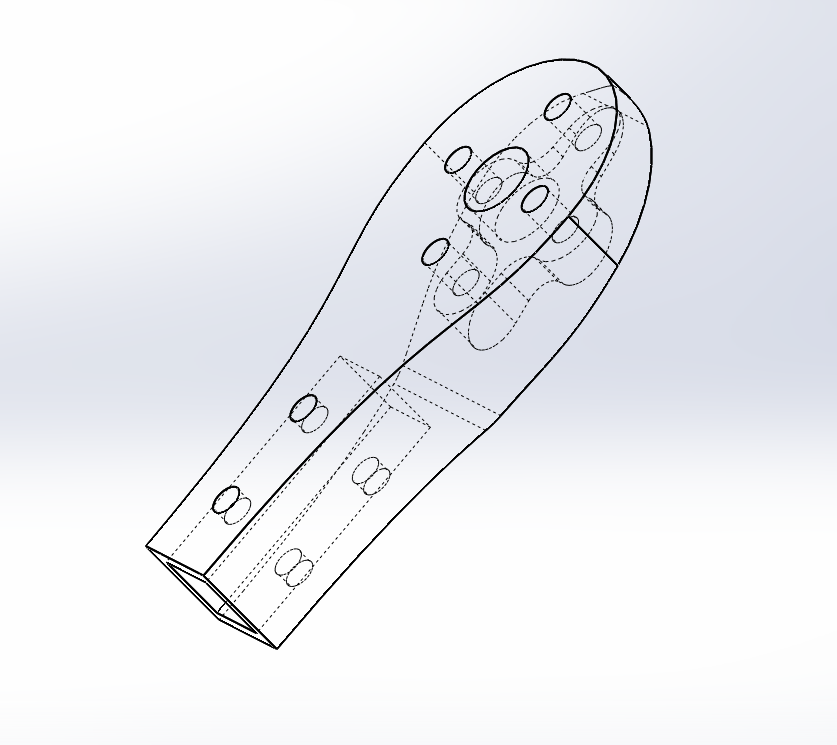
\includegraphics[width=0.6\textwidth]{hardware/portamotores}
		\caption{Portamotores en CAD }
		\label{portam}
	\end{figure}
	
	
	\item [$\bullet$] \textbf{Brazos}: se encargan de unir los portamotores con el \textit{núcleo} de la estructura. En este diseño, los brazos consisten en perfiles de aluminio de sección cuadrada de 8mm de lado.
	
	\item [$\bullet$] \textbf{Núcleo}: Es la pieza principal del diseño, en la que se anclan el resto de las partes y donde se alojan los componentes electrónicos. Esta pieza sustenta los brazos y el porta-baterias de la aeronave. Cuenta con agujeros a medida para poder situar el autopiloto y los variadores.
	
	\begin{figure}[htb!]
		\centering
		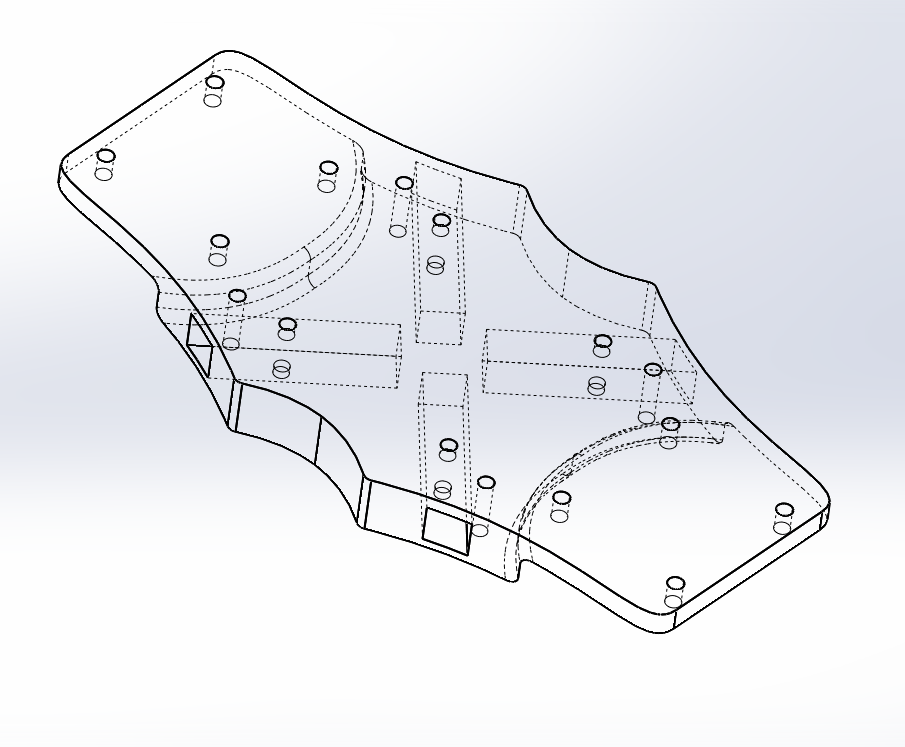
\includegraphics[width=0.8\textwidth]{hardware/base}
		\caption{Núcleo en CAD}
		\label{portam}
	\end{figure}
	 
	\item [$\bullet$] \textbf{Separadores}: su propósito es mantener unidos el \textit{núcleo} y el porta-baterías manteniendo una separación fija entre ellas.
	
	\begin{figure}[htb!]
		\centering
		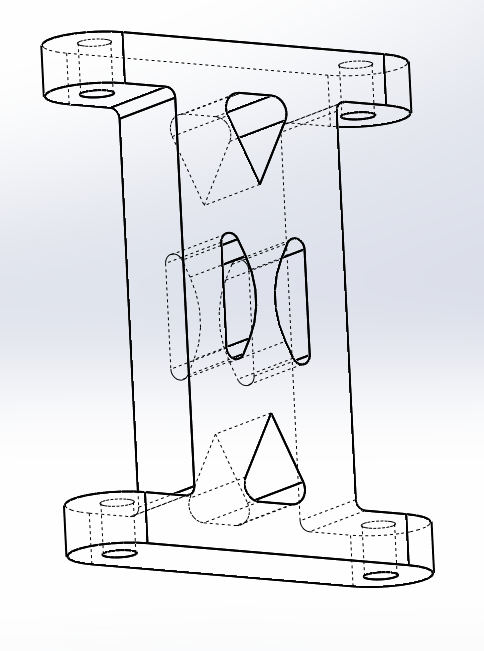
\includegraphics[width=0.4\textwidth]{hardware/union_base}
		\caption{Separadores en CAD}
		\label{portam}
	\end{figure}
	
	\item [$\bullet$] \textbf{Porta-baterías}: Es la parte inferior del cuadricóptero. En ella se apoya la batería Li-Po que alimenta al dron y se mantiene anclada durante el vuelo. Además posee unas protuberancias cuya función se asemejaría a las de un tren de aterrizaje.  
	
	\begin{figure}[htb!]
		\centering
		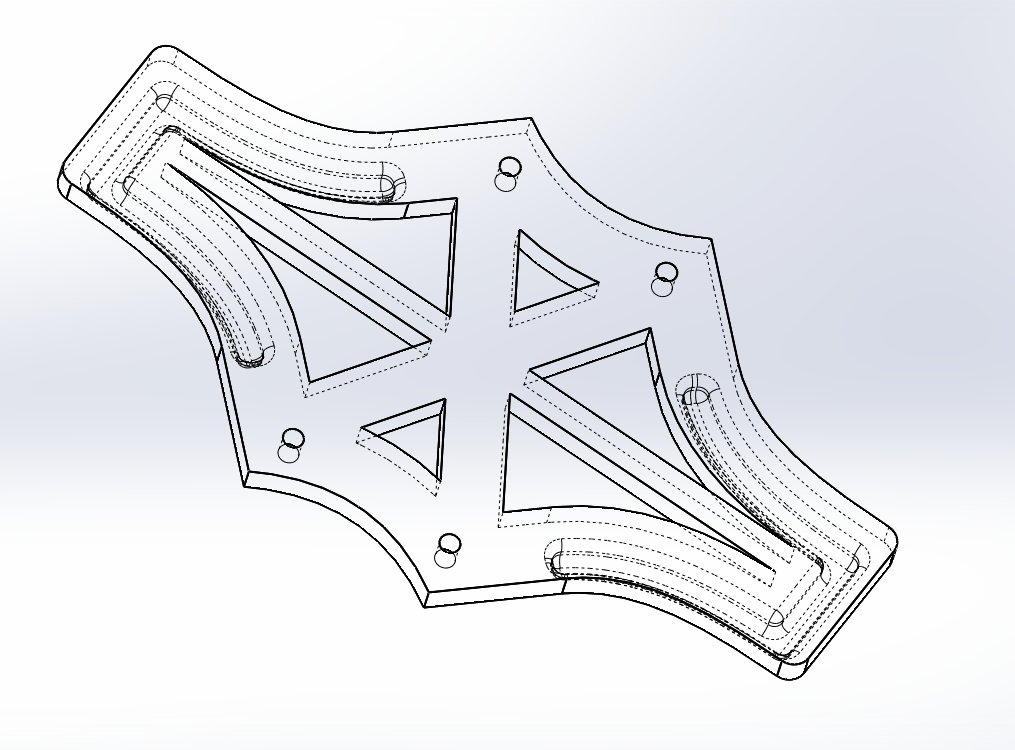
\includegraphics[width=0.8\textwidth]{hardware/lipo_support}
		\caption{Porta-baterías en CAD}
		\label{portam}
	\end{figure}
	
	  
\end{itemize} 

\section{Motores y hélices}
El dron cuenta con 4 motores sin escobillas (\textit{brushless}) LHI MT2204 II de 2300KV con una tensión de alimentación entre 7.2 V y 11.1 V (2s -3s en una batería LiPo) y una corriente continua máxima de 16A.

\begin{figure}[htb!]
	\centering
	\begin{subfigure}{0.4\textwidth}
		\centering
		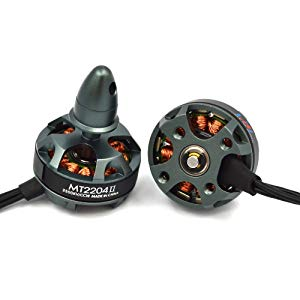
\includegraphics[height=0.2\textheight]{hardware/motores.jpg}
	\end{subfigure}
	\begin{subfigure}{0.4\textwidth}
	\centering
	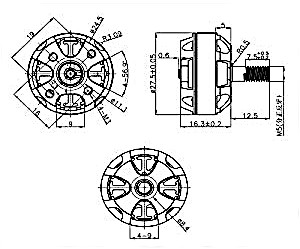
\includegraphics[height=0.2\textheight]{hardware/motoresPlanos}
\end{subfigure}
	\caption{Motores LHI MT2204 II empleados}
\label{hardware:motores}
\end{figure}

Se ha estimado que el peso aproximado de la aeronave se encuentra entorno a los 800 gramos. La literatura recomienda que los motores que se escojan deben tener empuje suficiente para poder levantar el doble del peso de la aeronave. Observando la tabla de especificaciones de los motores, se observa que, la hélice HQ5040 proporciona empuje suficiente con un ratio empuje/potencia bastante elevado, como se puede observar en la \cref{hardware:motoresTabla}.

\begin{figure}[htb!]
	\centering
	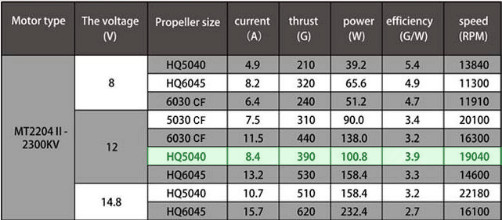
\includegraphics[width=0.7\textwidth]{hardware/MT2203_Table.jpeg}
	\caption{Tabla de especificaciones motor MT2204 II. }
	\label{hardware:motoresTabla}
\end{figure}

Es por esto que se han empleado hélices tripala HQ5040 de policarbonato y fibra de vidrio (\cref{hardware:helice}).

\begin{figure}[htb!]
	\centering
	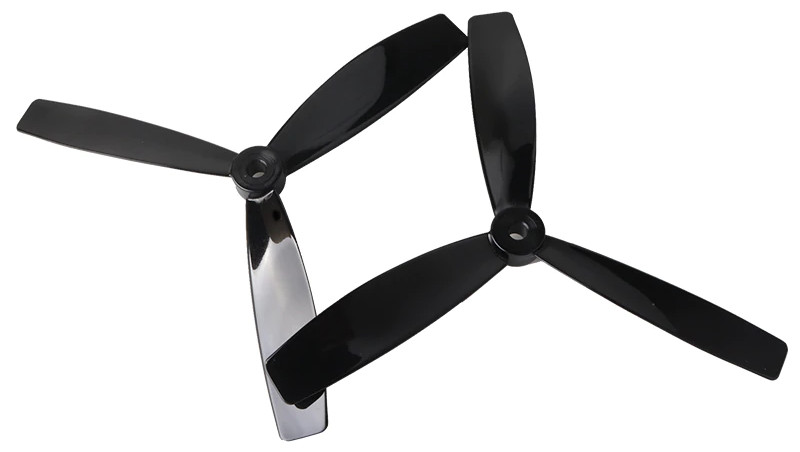
\includegraphics[width=0.5\textwidth]{hardware/helices.jpeg}
	\caption{Hélices tripala HQ5040}
	\label{hardware:helice}
\end{figure}

\section{Variadores (ESC)}


Los motores  que se han escogido son trifásicos, es decir, se alimentan con 3 corrientes alternas monofásicas de igual frecuencia y amplitud, desfasadas 120\grad \;eléctricos. Para obtener estás formas de ondas a partir de la corriente continua de las baterias, se utilizan los variadores.

Un variador o \textit{ESC (Electronic Speed Control)} es un circuito electrónico que se encarga de generar las ondas eléctricas necesarias para controlar y regular la velocidad de un motor eléctrico. Cuenta con un microcontrolador, el cual se encarga de conmutar los interruptores de potencia, con el ánimo de alimentar las distintas fases del motor de forma sincronizada, haciendo que gire a la velocidad deseada, veáse la \cref{hardware:esc_explicacion}.
\begin{figure}[htb!]
	\centering
	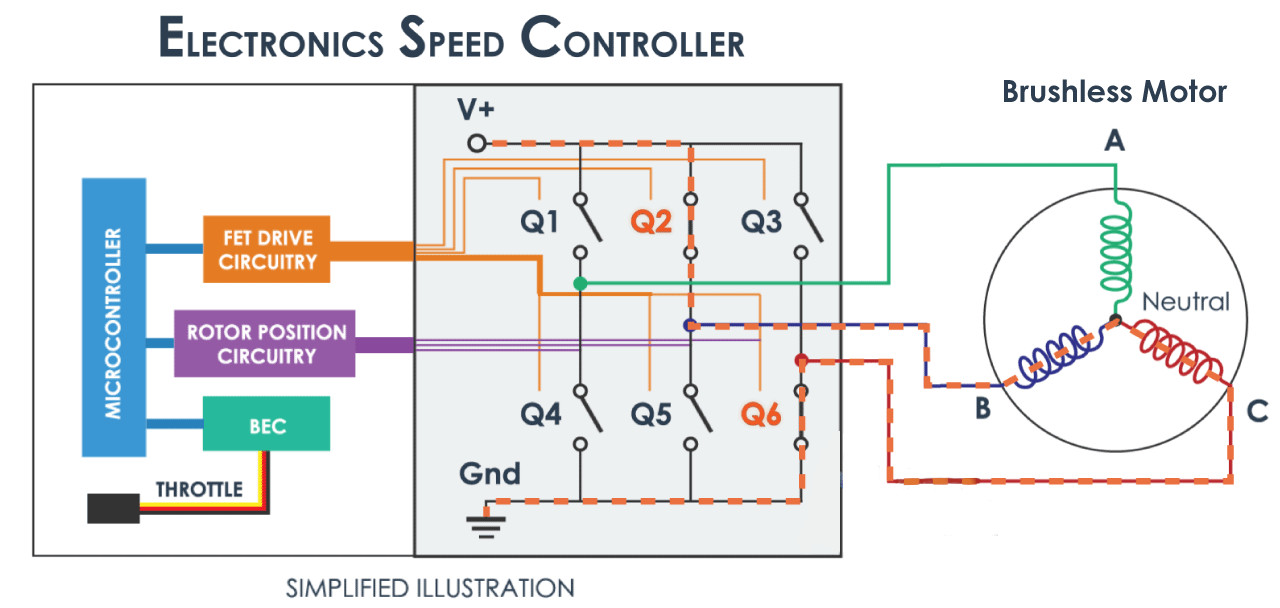
\includegraphics[width=0.6\textheight]{hardware/howtomecatronics}
	\caption{Funcionamiento ESC (www.howtomechatronics.com)}
	\label{hardware:esc_explicacion}
\end{figure}

Para el cuadricóptero se ha optado por emplear un variador BLHeli Multistar Race (\cref{hardware:esc}) que integra 4 variadores en uno, es decir se pueden alimentar 4 motores trifasicos con él. Estos variadores soportan una corriente de hasta 30 A cada uno.

\begin{figure}[htb!]
	\centering
	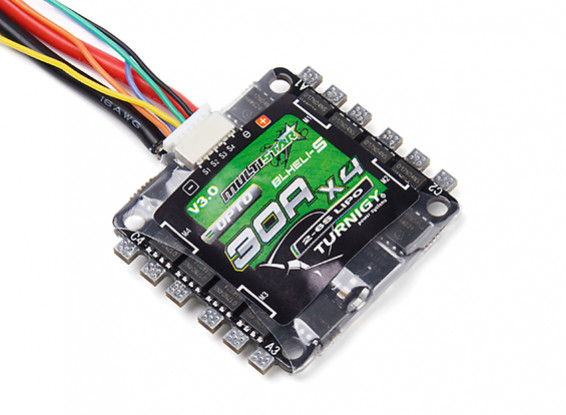
\includegraphics[width=0.5\textwidth]{hardware/esc.jpg}
	\caption{ESC Multistar Race 4 in 1 30A BLHeli empleado}
	\label{hardware:esc}
\end{figure}

\section{Baterías}
Para alimentar al dron, se han elegido baterías de litio-polímero (LiPo) de 3 celdas, lo que supone una tensión nominal de 11.1V (cada celda proporciona 2.7V). La tensión máxima que puede subministrar la batería es de 12.6V y la tensión mínima es de 9.6V. Si la tensión de alguna celda desciende de 3.2V la batería se puede dañar permanentemente. La batería escogida es una ZNACE de 3 celdas, con una capacidad de 5200mah y una tasa de descarga de 35C, por lo que es capaz de proporcionar una corriente de salida máxima de 5.2Ah $\cdot$ 35C = 182 A. La batería empleada cuenta con un conector XT60, por lo que el máximo de corriente que soporta en régimen continuo es de 60 A.

\begin{figure}[htb!]
		\centering
		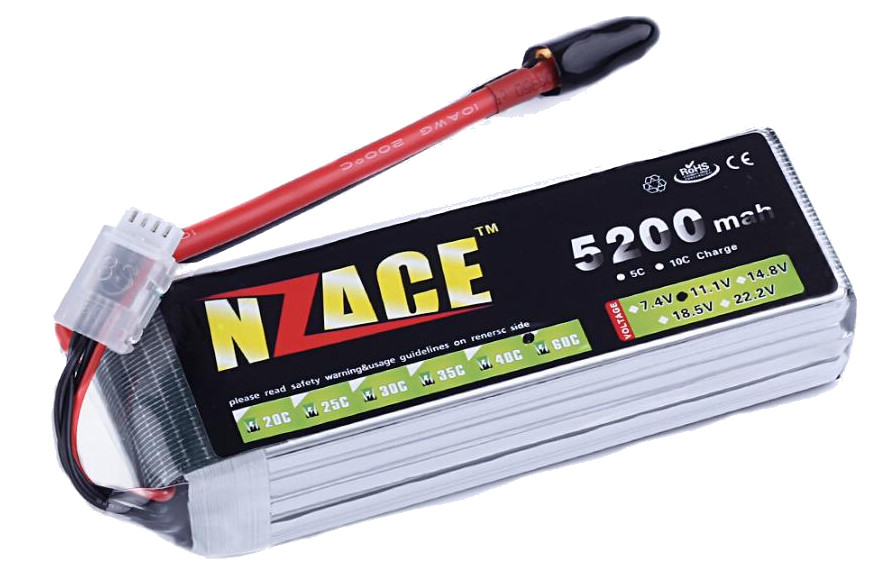
\includegraphics[width=0.5\textwidth]{hardware/bateriaNZACE}
		\caption{Batería LiPo 3s 35C 5200 mah de la marca NZACE empleada  }
		\label{hardware:Lipo}

\end{figure}


\section{Autopiloto}

En los drones, el sistema que se encarga de estabilizar al cuadricóptero y hacerlo pilotable se denomina la controladora de vuelo o el Autopiloto. Existe una gran variedad de controladoras en el mercado, pero para este trabajo se ha diseñado una controladora propia con el fin de poder tener acceso a todos los sensores y a implementar el algoritmo de control de forma óptima. El autopiloto consta de 3 partes diferenciadas: la electrónica de potencia, el microcontrolador y los sensores. A continuación \tb{se tratará} sobre estas partes con más detalle.\\



\begin{figure}[htb!]
	
	\centering
	\begin{subfigure}{0.49\textwidth}
		\centering
		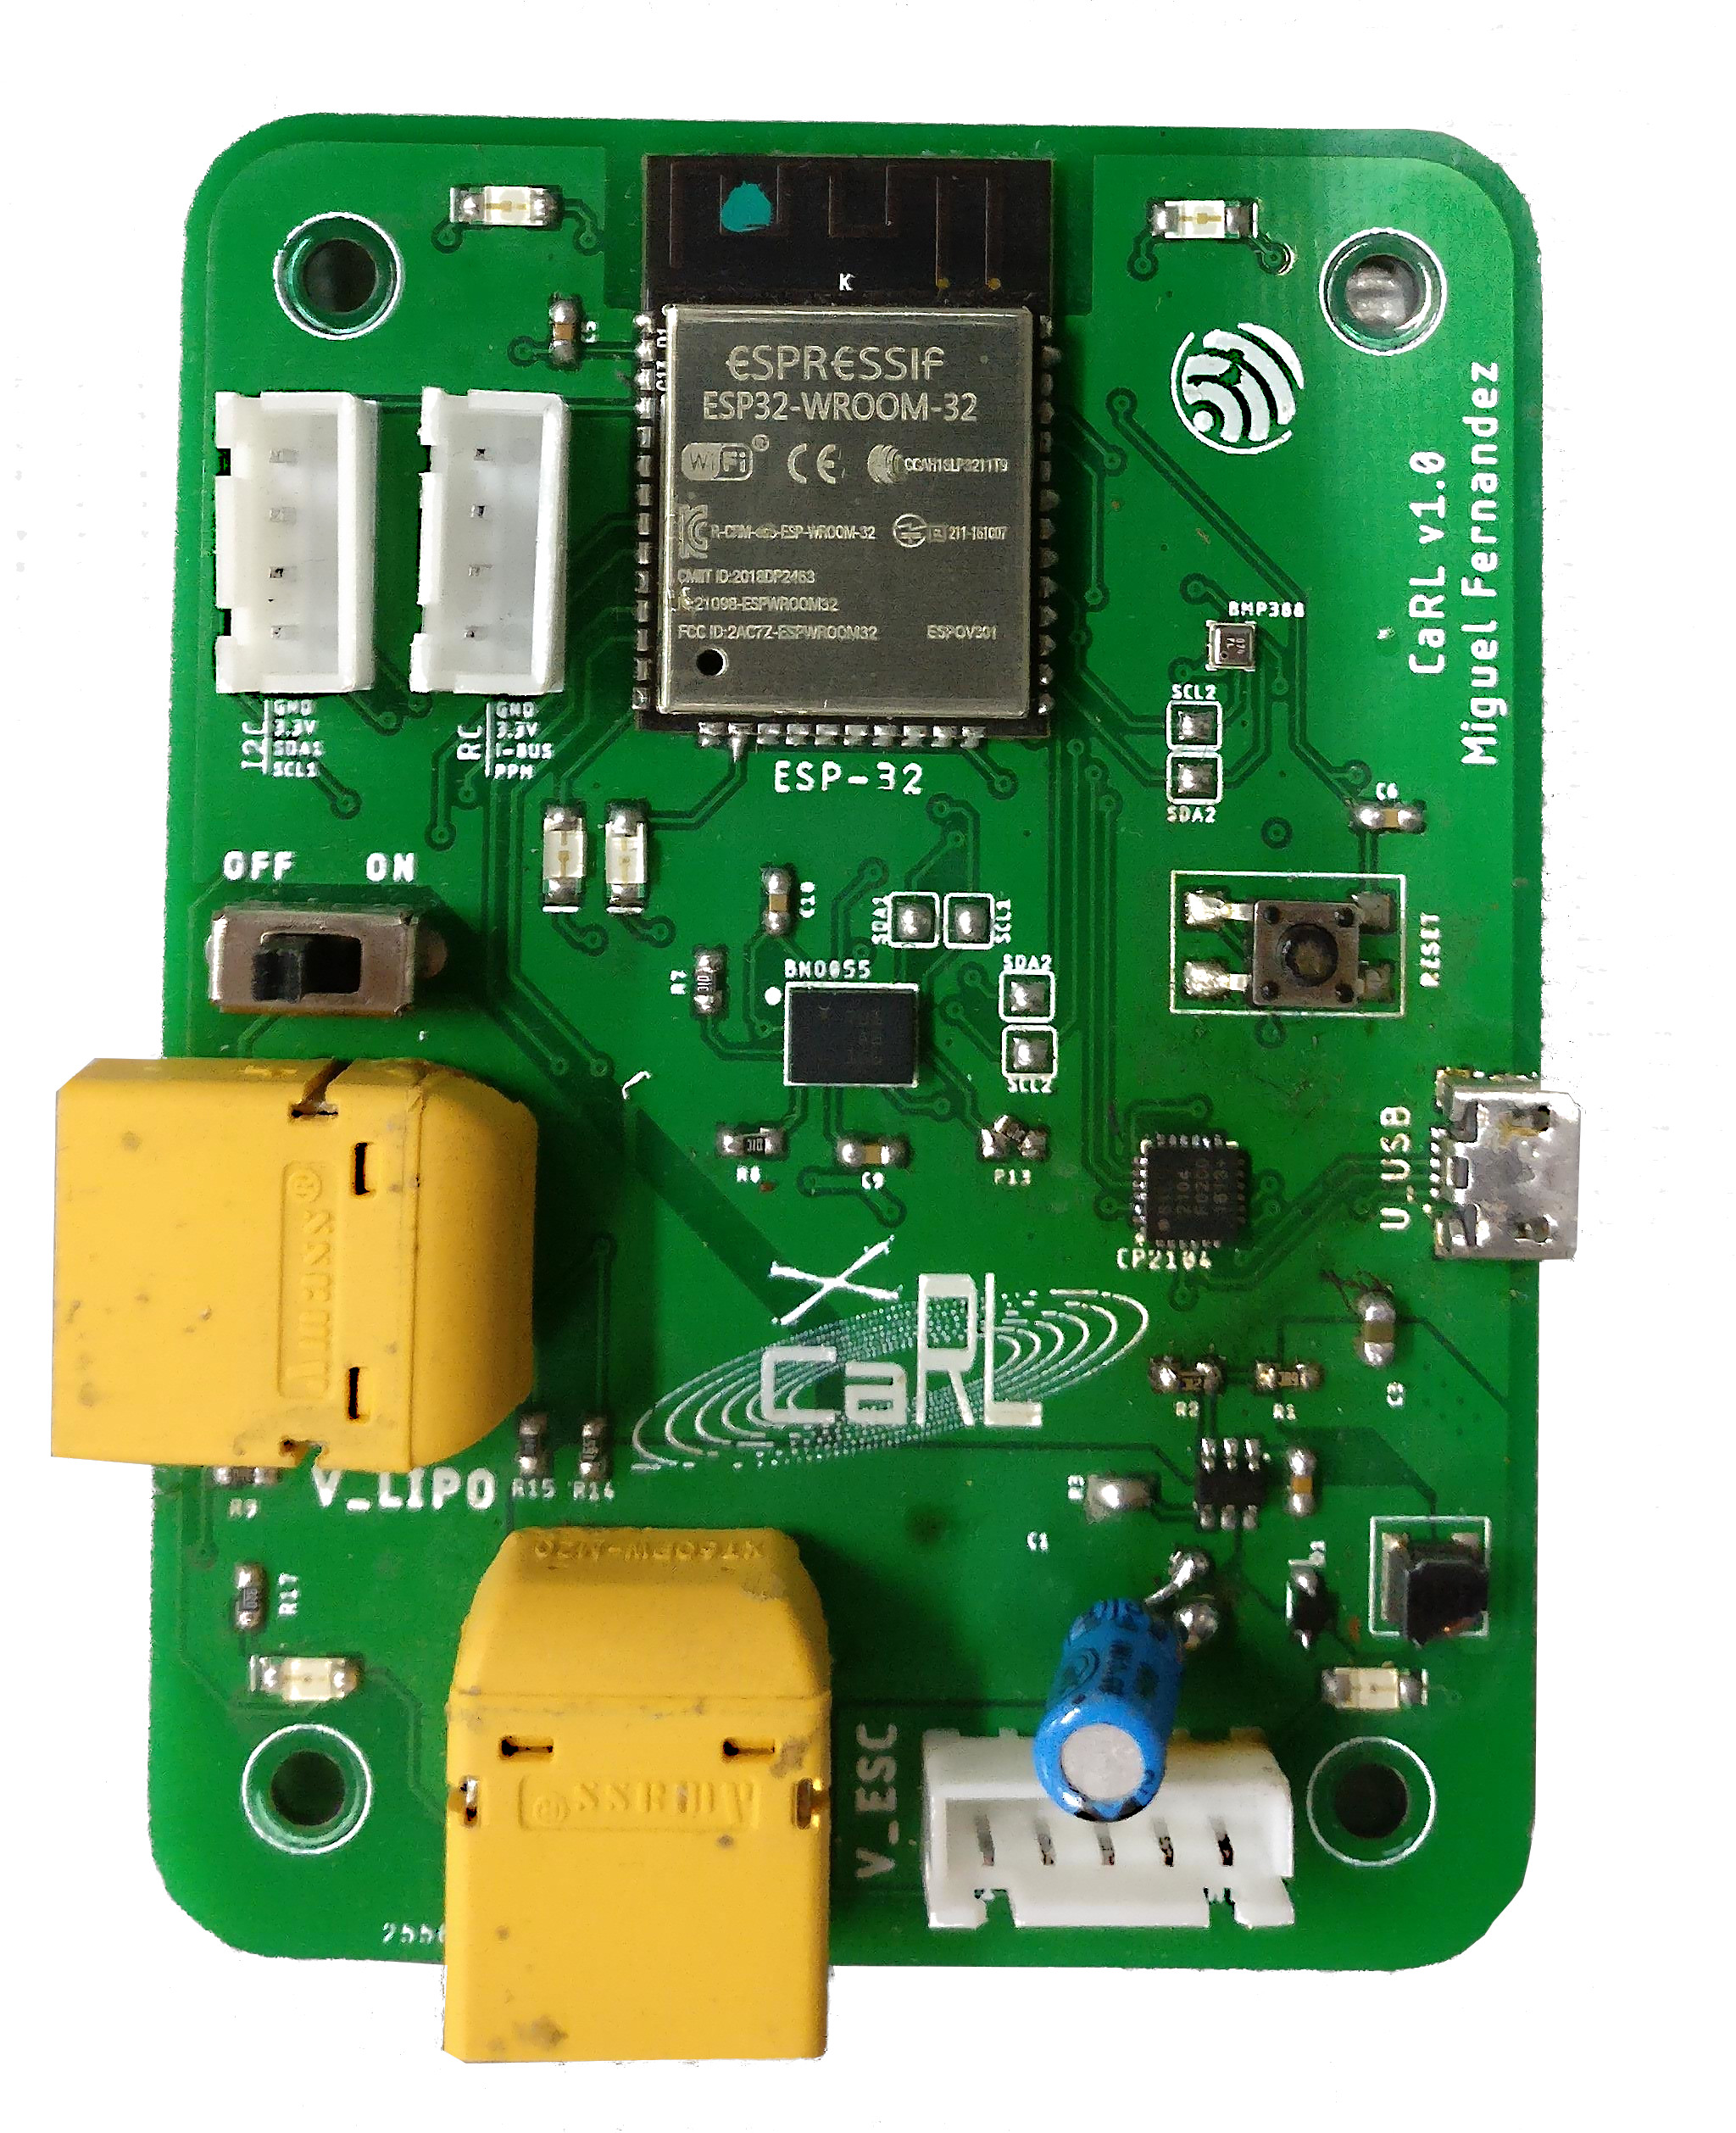
\includegraphics[height=1.2\textwidth]{hardware/AutopilotoFront}
	\end{subfigure}
	\begin{subfigure}{0.49\textwidth}
		\centering
		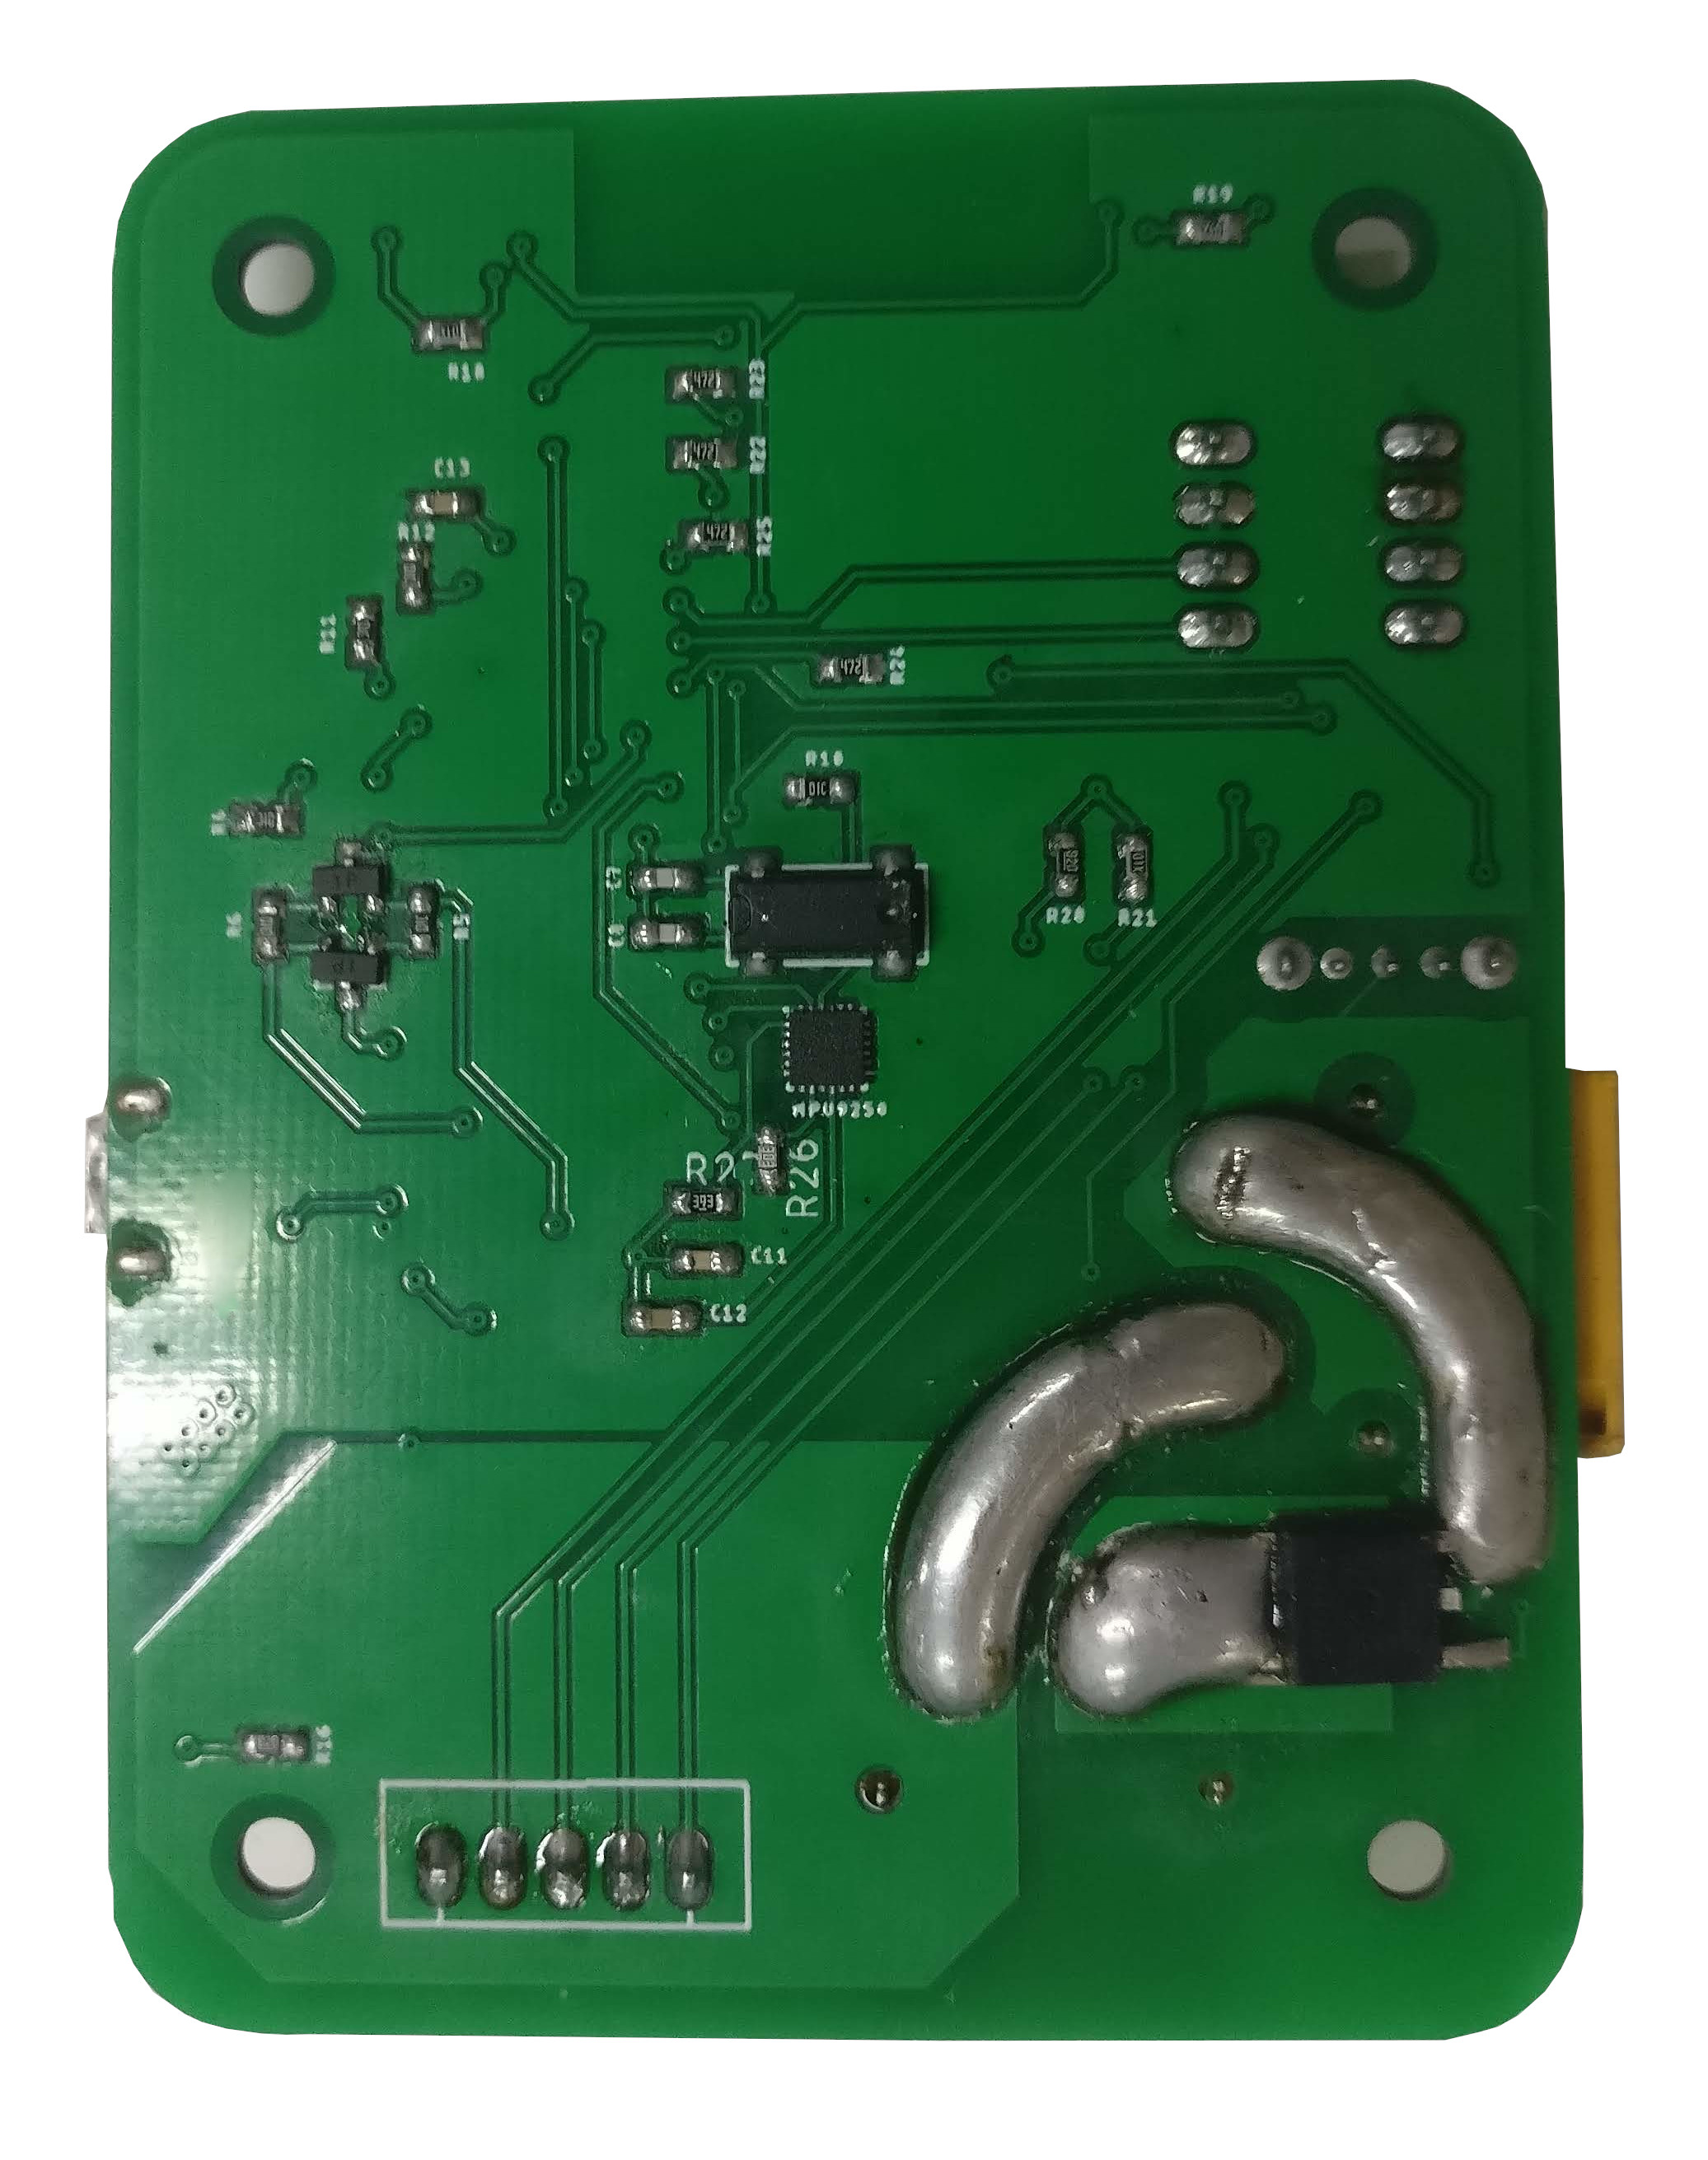
\includegraphics[height=1.2\textwidth]{hardware/AutopilotoBack}
	\end{subfigure}
	
	\caption{PCB autopiloto CaRL, anverso y reverso.}
	\label{PCB}
	
	
\end{figure}


\subsection{Fase de Potencia}

Con el fin de poder gestionar la potencia entregada por las baterías a la placa y a los motores se ha diseñado una etapa de potencia en la que se debe mencionar dos partes: el interruptor de potencia y el regulador a 3.3 Voltios.

\subsubsection{Interruptor de potencia}

Los motores del dron pueden llegar a consumir 12 Amperios cada uno, lo que los cuatro motores pueden llegar a consumir 48 Amperios. Un interruptor con tamaño reducido no puede manejar tanta corriente, por ello se ha empleado un transistor MOSFET de canal P por el que pueden circular hasta 100 Amperios, con el fin de abrir o cerrar el paso de corriente desde las baterías al resto de la placa. El MOSFET se controla con un interruptor de poca potencia entre drenador y puerta.Cuando se cierra el interruptor se alimenta directamente al ESC y al regulador de tensión.

Adicionalmente, a continuación del MOSFET se encuentra un divisor de tensión para poder medir la tensión de la batería a través del conversor analógico digital (ADC) del microcontrolador.   


\subsubsection{Regulador a 3.3V}

La eléctronica digital de la PCB se alimenta y emplea lógica a 3.3 Voltios, por lo que no la podemos conectar a las baterías de 11.1 Voltios.  Para adecuar la tensión se ha escogido un regulador Step-down de tipo Buck (Figura \ref{hardware:Buck}) \tb{(¿explico como funciona un convertidor Buck?)}. El circuito integrado que se encarga de conmutar la fuente es el chip AP3211.
\begin{figure}[htb!]
	\centering
		\begin{circuitikz}[american voltages,european resistors,scale=1]	
		
		\draw
		(0,2) to [V=$V_{in}$]  (0,-2)
		(0,2) to ++(1.5,0)
		++(0.5,0)node[nigfete,bodydiode,rotate=90]{}  to ++(2,0);
		
		\draw 
		(0,-2) to ++(4,0)
		++(0,0)[sD*] to ++(0,4)
		;
		\draw 
		(4,2) to [L=$L$,i=$i_L$] ++(3,0);
		\draw
		(7,2) to [C,l_=$C$] ++(0,-4)
		;
		
		\draw
		(7,2) to ++(3,0) 
		to [R =$R_{load}$,i=$i_{Load}$] ++(0,-4)
		to (0,-2)
		;
		\draw (2,0.75)node[]{\footnotesize SW};
		\draw (9.5,0.5)[short] to ++ (0,-0.5);
		\draw[-latex]
		(9.5,0)node[left] {$V_{out}$} to ++(0,-0.5);	
		
	\end{circuitikz}
	\caption{Esquema de un convertidor Buck}
	\label{hardware:Buck}
\end{figure}


\subsection{El microcontrolador (ESP32)}

El microcontrolador por el que se ha optado para este Autopiloto es el ESP32, un microcontrolador de doble núcleo con dos CPUs XTensaL6 con arquitectura Harvard \cite{ESP32TechnicalReference}. El ESP32 tiene una frecuencia de reloj de hasta 240MHz ,y cuenta con una antena WiFi a 2,4 GHz y conexión Bluetooth 4.2 BLE \cite{ESP32DataSheet}. Los motivos por los que se ha decidido emplear este microcontrolador son:
\begin{itemize}
	\item Elevada frecuencia de procesamiento y dos nucleos de procesamiento.
	\item Antena WiFi incorporada.
	\item Bajo consumo de potencia.
\end{itemize}

\par Para poder programar el microcontrolador se utiliza un convertidor USB (Bus Serie Universal) a UART (Transmisor-Receptor Asíncrono Universal) que permite conectar por USB el microcontrolador para poder programarlo y hacer depuración utilizando comunicaciones Serial. El chip que realiza esta funcion es el CP2104.

\subsection{Sensores}
La principal fuente de información procedente del exterior que recibe una controladora de vuelo se la proporcionan las unidades de medición inercial (IMU). Las IMUs son dispositivos electrónicos que son capaces de medir aceleraciones, velocidades y detectar la orientación de un sistema. El principal problema de estos sensores es que sufren error acumulativo a la hora de estimar posición y velocidad. Para corregir este error acumulativo en los drones, se suelen fusionar estas medidas con otras provenientes de mediciones absolutas tales como GPS o Láser, aunque en este autopiloto unicamente emplearemos las medidas de las IMUs.

\par Otros sensores utilizados frecuentemente en los autopilotos son brújulas (se encuentran integrados en la IMU para corregir errores de orientación) y barómetros (para estimar la altitud a la que se encuentra el dron).\\
\medskip

El autopiloto cuenta con dos IMUs de 9 Grados de Libertad y un barómetro para conseguir una mejor estimación del estado del cuadricóptero:

\begin{enumerate}
	\item \textbf{BNO 055 (BOSCH)}: El circuito integrado de Bosch es un sensor ``inteligente'' que incluye los sensores y la fusión de las lecturas de los distintos sensores en un único componente. Este encapsulado cuenta con: un acelerómetro, un giróscopo y un magnetómetro triaxial. Además integra un microcontrolador de 32 bits en el que se ejecuta el algoritmo de fusión integrado. El sensor se encuentra en un encapsulado LGA de 28 pines con una huella (\textit{footprint}) de $3,8$ x $5.2\; mm^2$.
	
	Este sensor nos proporciona estimaciones del estado completo de la aeronave con una frecuencia de refresco de 100Hz. 
	
	\item \textbf{MPU 9250 (TDK InvenSense)}: El sensor inercial de TDK es un módulo multichip compuesto por un MPU6050 (Contiene un accelerómetro y un giróscopo triaxial con un \textit{procesador digital de movimiento} (DMP)) y un  AK8963 (un magnetómetro digital triaxial). El sensor posee un encapsulado QFN de 3x3x1 $mm$ con 24 pines.
	
	Este dispositivo nos proporciona medidas del accelerometro y el giróscopo a una frecuencia superior al BNO055 pero con una estimación peor de los angúlos que el dispositivo de BOSCH.
	
	\item \textbf{BMP388 (BOSCH)}: El BMP388 es un barómetro digital de 24 bits con bajo consumo y bajo ruido. Se encuentra en un encapsulado LGA de 10 pines de dimensiones 2 x 2 x 0,75 $mm3$.
	
	Aunque el autopiloto cuenta con este sensor, éste no se ha utilizado en este trabajo debido a que no se tiene en cuenta la altitud en los controladores.
	
\end{enumerate}

	
\begin{figure}[htb!]
	\centering
	\begin{subfigure}{0.4\textwidth}
		\centering
		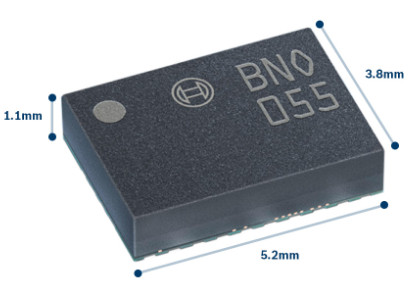
\includegraphics[height=0.5\textwidth]{hardware/bno055.jpeg}
	%	\caption{Sensor BNO055}
		\label{BNO055}
	\end{subfigure}
	\begin{subfigure}{0.4\textwidth}
		\centering
		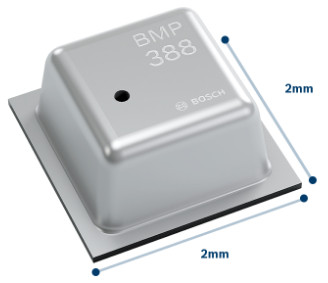
\includegraphics[height=0.5\textwidth]{hardware/bmp388.jpeg}
	%	\caption{Sensor BMP388}
		\label{BMP388}
	\end{subfigure}
	\caption{Sensores BNO055 y BMP388 respectivamente}
\end{figure}


 
%\section{Otros (Receptora radio)}

\section{Banco de pruebas}
Para poder realizar la experimentación real de forma segura, se han diseñado distintas estructuras para poder sujetar al cuadricóptero permitiéndole rotar con distintos grados de libertad (GdL) en función de la estructura. Estas uniones han permitido poder probar distintos controladores de forma segura y controlada.


Se pueden distinguir 2 tipos de estructuras en función de sus grados de libertad:

\begin{itemize}
	\item \textbf{Rótulas con 1 único grado de libertad}: Para las primeras pruebas de los reguladores es fundamental poder descomponer el control en problemas más sencillos, en este caso permitiendo al sistema rotar en 1 grado de libertad. Se han construido 2 versiones de la misma rótula, una permite el movimiento en Pitch y la otra lo permite en Roll. Esto permite desacoplar los bucles de control y poder probar distintos algoritmos de control.
	
	
	\begin{figure}[htb!]
		\centering
		\begin{subfigure}{0.4\textwidth}
			\centering
			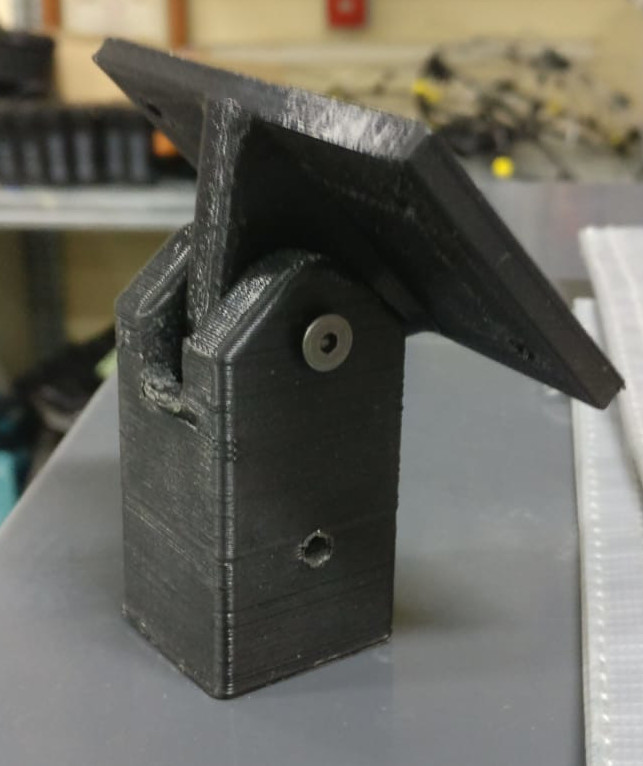
\includegraphics[width=0.8\textwidth,height=0.2\textheight]{hardware/rotulaPitch1.jpeg}
			\caption{Motores LHI MT2204 II empleados}
			\label{a}
		\end{subfigure}
		\begin{subfigure}{0.4\textwidth}
			\centering
			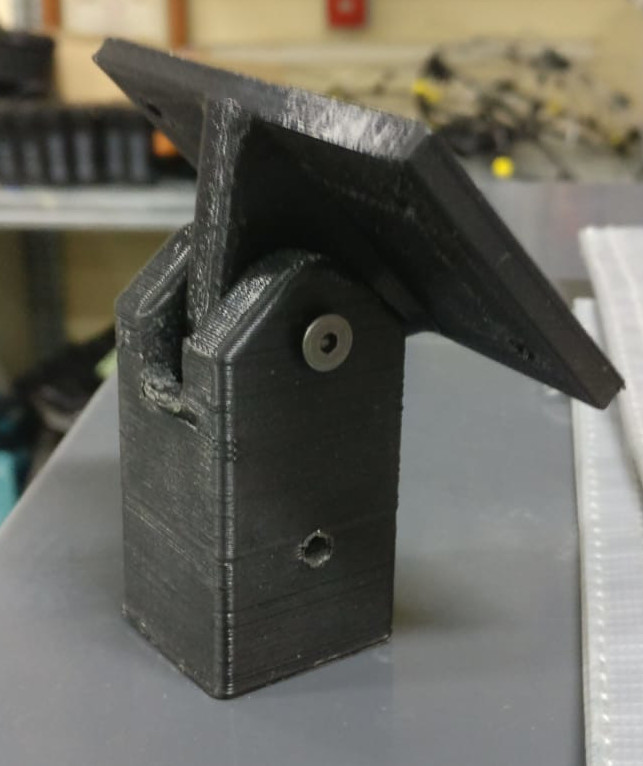
\includegraphics[width=0.8\textwidth,height=0.2\textheight]{hardware/rotulaPitch1.jpeg}
			\caption{ESC Multistar Race 4 in 1 30A BLHeli empleado}
			\label{b}
		\end{subfigure}
	\end{figure}

	Estas uniones son sencillas y robustas lo que nos da seguridad a la hora de poder probar y ajustar los reguladores.
	Las restricciones de movimiento de estas uniones permiten rotaciones de $\pm 60\degree$ en el angulo permitido.
	
	
	\item \textbf{Rótula con múltiples grados de libertad}: Después de conseguir estabilizar al cuadricóptero en pitch y en roll de forma individual la siguiente aproximación consiste en emplear rotulas con 3 GdL. Sobre estas uniones también se han realizado 2 versiones. La primera consta de una única rotula con sus 3 grados de libertad con restricciones de movimiento de:
	
	\begin{align*}
	-60 \degree &\le \varphi \le 60\degree \quad \;\;\;  \text{Roll}\\ 
	-60 \degree&\le \theta \le 60\degree \qquad  \text{Pitch} \\
	-180 \degree&\le \psi \le 180\degree\quad \;  \text{Yaw}
	\end{align*}
	
	
	La segunda consta de acoplar 2 juntas esféricas como las anteriores una a continuación de la otra, lo que permite, además de disminuir las restricciones de movimiento en las rotaciones, pequeños desplazamientos en el espacio tridimensional.
	
	\begin{figure}[htb!]
		\centering
		\begin{subfigure}{0.4\textwidth}
			\centering
			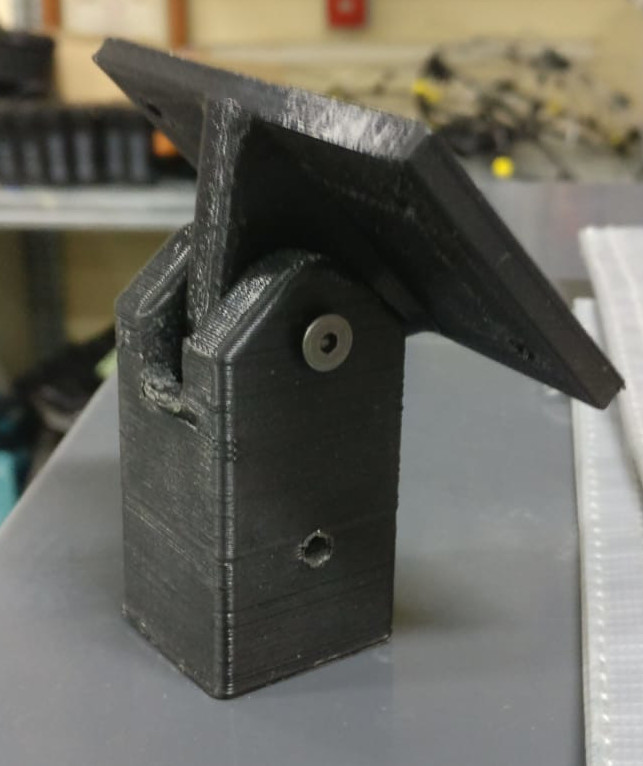
\includegraphics[width=0.8\textwidth,height=0.2\textheight]{hardware/rotulaPitch1.jpeg}
			\caption{Motores LHI MT2204 II empleados}
			\label{c}
		\end{subfigure}
		\begin{subfigure}{0.4\textwidth}
			\centering
			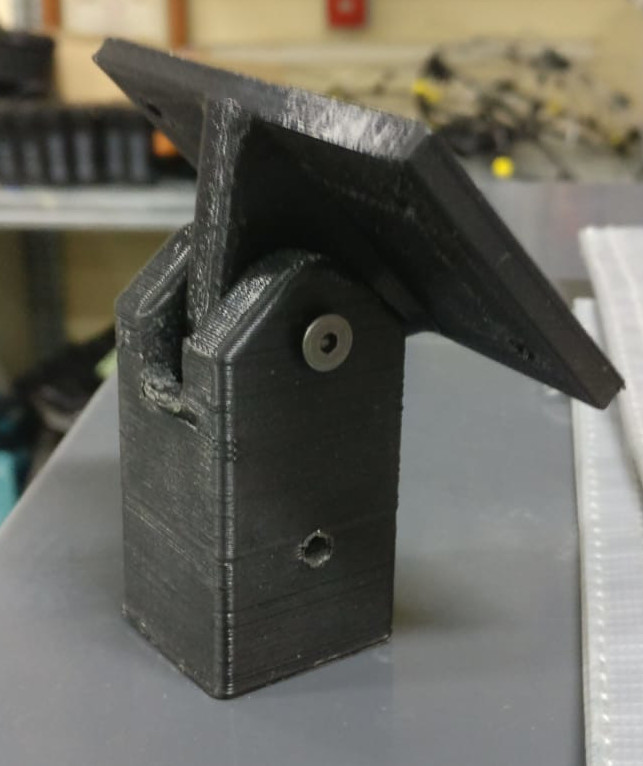
\includegraphics[width=0.8\textwidth,height=0.2\textheight]{hardware/rotulaPitch1.jpeg}
			\caption{ESC Multistar Race 4 in 1 30A BLHeli empleado}
			\label{d}
		\end{subfigure}
	\end{figure}
	
	
	
\end{itemize}


\tb{\huge imagen rotulas y/o CAD }


